%
% File STS_SemEval.tex
%

\documentclass[11pt,letterpaper]{article}
\usepackage{naaclhlt2016}
\usepackage{times}
\usepackage{latexsym}
\usepackage{multirow}
\usepackage{amsmath}
\usepackage{tikz}
% Optional PGF libraries
\usepackage{pgflibraryarrows}
\usepackage{pgflibrarysnakes}
\naaclfinalcopy % Uncomment this line for the final submission
\def\naaclpaperid{***} %  Enter the naacl Paper ID here

% To expand the titlebox for more authors, uncomment
% below and set accordingly.
% \addtolength\titlebox{.5in}

\newcommand\BibTeX{B{\sc ib}\TeX}
\newcommand{\tabincell}[2]{\begin{tabular}{@{}#1@{}}#2\end{tabular}}

\title{ECNU at SemEval-2016 Task 1: Leveraging Word Embedding from Macro and Micro Views to Boost Performance for Semantic Textual Similarity} %\Thanks{.}}

\author{Junfeng Tian$^{1}$, Man Lan$^{1,2\ast}$\\
        $^1$Department of Computer Science and Technology,\\
        East China Normal University, Shanghai, P.R.China \\
        $^2$Shanghai Key Laboratory of Multidimensional Information Processing \\
        {\tt 51151201048@ecnu.cn, mlan@cs.ecnu.edu.cn$^{\ast}$} \\
}
\date{}

\begin{document}

\maketitle
\begin{abstract}

This paper presents our submissions for semantic textual similarity task in SemEval 2016. Based on several traditional features (i.e., string-based, corpus-based, machine translation similarity and alignment metrics), we leverage word embedding from macro (i.e., first get representation of sentence, then measure the similarity of sentence pair) and micro views (i.e., measure the similarity of word pairs separately) to boost performance. Due to the various domains of training data and test data, we adopt three different strategies: 1) U-SEVEN: an unsupervised model, which utilizes seven straight-forward metrics; 2) S1-All: using all available datasets; 3) S2: selecting the most similar training sets for each test set. Results on test sets show that the unified supervised model (i.e., S1-All) achieves the best averaged performance with a mean correlation of 75.07\%.

\end{abstract}

\section{Introduction}
\label{sec:introduction}

Estimating the degree of semantic similarity between two sentences is the building block of many Natural Language Processing (NLP) applications, such as question answering, textual entailment, text summarization etc. Therefore, Semantic Textual Similarity (STS) has received an increasing amount of attention in recent years, e.g., the STS tasks in Semantic Evaluation Exercises have been held from 2012 to 2016.

To identify semantic similarity of sentence pairs, most existing works adopt at least one of the following feature types: 1) string based similarity \cite{bar2012ukp,jimenez2012soft} which employs common functions to calculate similarities over string sequences extracted from original strings, e.g., lemma, stem, or $n$-grams sequences; 2) corpus based similarity \cite{saric2012takelab} where distributional models such as Latent Semantic Analysis (LSA), are used to derive the distributional vectors of words from a large corpus according to their occurrence patterns, afterwards, similarities of sentence pairs are calculated using these vectors; 3) knowledge based method \cite{DBLP:journals/corr/AgirreBS15} which estimates the similarities
with the aid of external resources, such as WordNet. Among them, \newcite{sultan-bethard-sumner:2015:SemEval} leverage different word alignment strategies to bring word-level similarity to sentence-level similarity.

%move to introduction
Traditional NLP feature engineering often treat sentence as a bag of words or term frequency, and endeavor to evaluate the similarity according to the co-occurrence of words or other replacement words. For example, \newcite{zhao-zhu-lan:2014:SemEval} built a supervised model using ensemble of heterogeneous features and achieved great performance on STS Task 2014. However, it is difficult to evaluate semantic relatedness if all the word in both sentences is unique. For example:  {\em A storm will spread snow over Shanghai; The earthquakes have shaken parts of Oklahoma}. These sentences have no words in common, although they convey the similar information.

%{\color{red} TODO: our work of word embedding}
In this work, we first borrow the aforementioned effective types of similarity measurements including string-based, corpus-based, machine translation similarity and alignment measures to capture the semantic similarity between two sentences. Besides, we also present our highly interpretable and hyper-parameter free word embedding features from macro and micro views to boost the performance. Then we adopt three different strategies of the usage of training data: 1) U-SEVEN: an unsupervised model, which utilizes seven straight-forward metrics (i.e., longest common sequence, alignment feature, corpus-based feature, and others are all from word embedding features); 2) S1-All: use all available datasets and train a unified regression model after deleting unnecessary features; 3) S2: select the most similar training sets for each test set, according to the source of the dataset, average sentence length, and similarity distance (i.e., word mover's distance, discussed in Section \ref{ssec:word embedding feature engineering}).

%system we developed last year. Besides, we also present different features like Shallow Similarity Features, Knowledge-based Features, Alignment Features and Word Embedding Features.

The rest of this paper is organized as follows. Section 2 describes various similarity measurements used in our systems. Section 3  gives the datasets and system setups. Results on training set and test set will show in Section 4 and 5 respectively, and finally conclusion is given in Section 6.

\section{Semantic Similarity Measurements}

%section overview
%what we do and why we do

Previous excellent work \cite{zhao-zhu-lan:2014:SemEval,sultan-bethard-sumner:2015:SemEval} have shown great performance for STS tasks. Following their works, we engineer the traditional widely used features for semantic similarity measurements (i.e., string-based, corpus-based, machine translation similarity and alignment measures). In this work, we also present our highly interpretable and hyper-parameter free word embedding features from macro and micro views to boost the performance.

\subsection{Preprocessing}
Several text preprocessing operations are performed before feature engineering:
1) Converting the contractions to their formal writing, e.g., {\em ``doesn't"} is rewritten as {\em ``does not"}.
2) The WordNet-based Lemmatizer implemented in Natural Language Toolkit\footnote{http://www.nltk.org} is used to lemmatize all words to their nearest based forms in WordNet, e.g., {\em ``was"} is lemmatized to {\em ``be"}.
3) Stanford CoreNLP \cite{manning-EtAl:2014:P14-5} is adopted to get the Part-Of-Speech (POS) tag and Named Entity Recognition (NER) tag.

\subsection{Traditional NLP Feature Engineering}
\label{ssec:traditional nlp feature engineering}

\subsubsection{String-Based Similarity}
%{\bf ECNU:} This set of feature is taken from our previous work \cite{zhao-lan-tian:2015:SemEval}.
{\bf Length Features (len):} We record the length information of given sentence pairs using the following eight measure functions: $|A|, |B|, |A-B|, |B-A|, |A \cup B|, |A \cap B|, \frac{|A-B|}{|B|}, \frac{|B-A|}{|A|}$, where $|A|$ stands for the number of non-repeated words in sentence $A$.

{\bf Syntactic Features (pos):} Since two sentences with similar syntax structure convey similar meaning, we estimate the similarities of syntax structure. We firstly use Stanford CoreNLP toolkit \cite{manning-EtAl:2014:P14-5} to obtain the POS tags of each sentence. Afterwards, we use eight measure functions mentioned in the Length Features on the sets of POS tags to calculate Syntactic Features.

{\bf Longest Common Sequence (lcs):} In consideration of the different length of sentence pairs, we divide the maximum length of the common subsequence of two sentences by the length of the shorter one.

{\bf {\em n}-grams Overlap Features ({\em n}-grams):} We obtain $n$-grams at three different level (i.e., the original word level, the lemmatized word level and the character level). Then Jaccard similarity is used for calculating the similarity of these $n$-grams pairs. In our experiments, $n = \{1, 2, 3\}$ are used for the word level whereas $n = \{2, 3, 4\}$ are used for the character level.

{\bf Named Entities Features (ner): } Besides of the surface similarities between words, we also calculate the relatedness of named entities in two sentences using {\em lcs} function. Seven types of named entities (i.e., {\em location, organization, data, money, person, time, percent}), recognized by Stanford CoreNLP toolkit \cite{manning-EtAl:2014:P14-5}, are considered.
%{\bf Difference Features (diff):} We have paid more attention to the match features than the difference of the two sentences. Not only the more similarity causes the score is more high, but also the less difference make the score more high.
%We checked whether the negative terms happens in each sentences and set this feature is 1 if it contains the negative terms on the negative list. What is more, removed the match words, we calculate the WordNet path similarity between the words.

%{\bf WordNet Augment Word Overlap (overlap):} To allow for some lexical variation, WordNet is used to assign partial scores
%to words tha are not common to both sentences and the path length represent the similarity score.

%{\bf Other Features (others):} Some other features significantly improve the  performance. Numbers Overlap Feature catch the number difference in the two sentences, Named Entity features(ner) can tell us that if the same Entity in the two sentence, They may describe the the same thing, while the length of the sentences can normalized differences in the two sentence pair.


\subsubsection{Machine Translation Similarity}

Machine Translation (MT) evaluation metrics are designed to assess whether the output of a MT system is semantically equivalent to a set of reference translations. The two given sentences are viewed as one input and one output of a MT system, then we get two MT scores of each MT measure (i.e., {\em WER, TER, PER, NIST, ROUGE-L, GTM-1}).
Two strategies is employed to get MT similarity features, 1). average two MT scores in each MT measure; 2). concatenate two MT scores  in each MT measure.

\subsubsection{Corpus-based Features}

{\bf WordNet Rank Features (wordnet):} The above semantic similarities only consider the surface similarities rather than their relations in corpus. Hence, we use graph-based lexical relatedness, which performs with a pre-existing Knowledge Base (KB) (i.e., WordNet), to get the relations of words. Then Personalized PageRank is applied on the Lexical Knowledge Base (LKB) to rank the vertices of the LKB. The details of the method are described in \newcite{DBLP:journals/corr/AgirreBS15}. It outputs a ranking vector of the sentence over KB nodes and the values of the weights are normalized so that all link weights of particular headword sum to one. Finally, we calculate the {\tt Cosine, Manhattan, Euclidean, Jaccard} of the two sentence vectors.

{\bf Vector Space Sentence Similarity (lsa):} This measure is motivated by the idea of compositionality of distributional vector \cite{mitchell-lapata:2008:ACLMain}. we adopt two distributional word sets released by TakeLab \cite{saric2012takelab}, where Latent Semantic Analysis (LSA) was performed on the New York Times Annotated Corpus (NYT)\footnote{https://catalog.ldc.upenn.edu/LDC2008T19} and Wikipedia. Then two strategies are used to convert the distributional meaning of words to sentence level: 1). simply summing up. 2). using {\em tf} to weigh each word vector.


\subsubsection{Alignment Measures}
\cite{sultan-bethard-sumner:2015:SemEval} used delicate word aligner to compute proportion of aligned words across the two input sentences. It aligned words based on their semantic similarity in the two sentences, as well as the similarity between local semantic contexts, which relies on dependencies and surface-form neighbors. The paraphrase Database (PPDB) \cite{ganitkevitch2013ppdb} was used to identify semantically similar words. Word pairs are aligned with greedy strategy, in descending order of their similarity.

{\bf Global Alignment Features (global):} Given sentences $S_1$ and $S_2$, single proportion over all words is computed over all words:
\begin{equation}
\footnotesize
\begin{aligned}
sim(S_1, S_2) = \frac{n_a(S_1) + n_a(S_2)}{n(S_1)+n(S_2)}
\end{aligned}\label{eq:align}
\end{equation}
where $n(S_i)$ is the number of non-repeated words in $S_i$, while $n_a(S_i)$ is the number of aligned content words in $S_i$.

{\bf Specific Alignment Features (pos-specific):} Taking weight of POS tag of aligned words into consideration, score of aligned {\em noun} word pair is surely higher than the {\em adjective}. Using this property, we propose the specific alignment feature, to calculate the aligned words proportion specifically according to POS tag (i.e., noun, verb, adjective, adverb).

\subsection{Word Embedding Feature Engineering}
\label{ssec:word embedding feature engineering}
%neural network achieve great success, % we want to use it to get semantic relateness(example) %Formula
Recently, the distributed representations of words (i.e., word embedding) learned by neural networks over a large raw corpus have been shown that they performed significantly better than Latent Semantic Analysis for preserving linear regularities among words \cite{mikolov2013distributed}. The training on very large datasets allows the model to learn complex word relationships such as $vec(Berlin) - vec(Germany) + vec(France) \approx vec(Paris)$ \cite{mikolov2013distributed}.

\begin{figure}[b]
\small
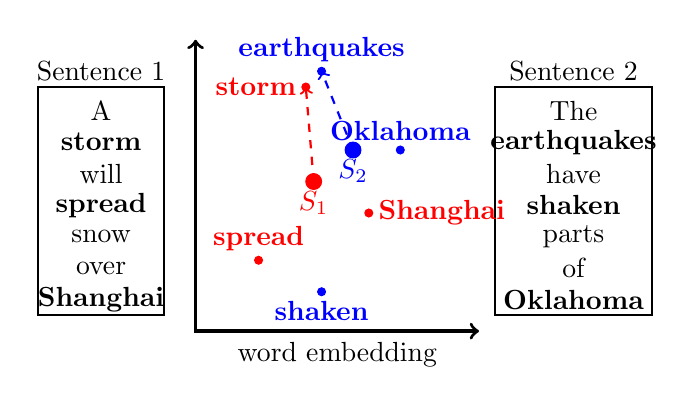
\begin{tikzpicture}
\draw [thick] (0.2, 0.5) rectangle (1.8, 3.4);
\draw [very thick, <->] (2.2, 4.0) -- (2.2, 0.3) -- (5.8, 0.3);
\draw [thick] (6.0, 0.5) rectangle (8.0, 3.4);

\node at (4.0, 0.0) {word embedding};

\node at (1.0, 3.6) {Sentence 1};
\node at (1.0, 3.1) {A};
\node at (1.0, 2.7) {\bf storm};
\node at (1.0, 2.3) {will};
\node at (1.0, 1.9) {\bf spread};
\node at (1.0, 1.5) {snow};
\node at (1.0, 1.1) {over};
\node at (1.0, 0.7) {\bf Shanghai};

\node at (7.0, 3.6) {Sentence 2};
\node at (7.0, 3.1) {The};
\node at (7.0, 2.7) {\bf earthquakes};
\node at (7.0, 2.3) {have};
\node at (7.0, 1.9) {\bf shaken};
\node at (7.0, 1.5) {parts};
\node at (7.0, 1.1) {of};
\node at (7.0, 0.7) {\bf Oklahoma};

\draw [fill, red] (3.6, 3.4) circle [radius=0.05];
\node [left, red] at (3.6, 3.4) {\bf storm};

\draw [fill, blue] (3.8, 3.6) circle [radius=0.05];
\node [above, blue] at (3.8, 3.6) {\bf earthquakes};

\draw [fill, red] (3.0, 1.2) circle [radius=0.05];
\node [above, red] at (3.0, 1.2) {\bf spread};

\draw [fill, blue] (3.8, 0.8) circle [radius=0.05];
\node [below, blue] at (3.8, 0.8) {\bf shaken};

\draw [fill, red] (4.4, 1.8) circle [radius=0.05];
\node [right, red] at (4.4, 1.8) {\bf Shanghai};

\draw [fill, blue] (4.8, 2.6) circle [radius=0.05];
\node [above, blue] at (4.8, 2.6) {\bf Oklahoma};


\draw [fill, red] (3.7, 2.2) circle [radius=0.1];
\node [below, red] at (3.7, 2.2) {\bf $S_1$};

\draw [fill, blue] (4.2, 2.6) circle [radius=0.1];
\node [below, blue] at (4.2, 2.6) {\bf $S_2$};

\draw [->, blue, dashed, thick] (4.2, 2.6) -- (3.8, 3.6);
\draw [->, red, dashed, thick] (3.7, 2.2) -- (3.6, 3.4);
\end{tikzpicture}
\caption{An illustration of the word centroid distance. Points in red is the word from sentence 1 (stopwords is ignored), while blue from sentence 2. $S_i$ is the centroid of points from sentence i.}\label{fig:wcvd}
\end{figure}

As discussed in Section \ref{sec:introduction}, it is very hard to evaluate semantic similarity if no words in the sentence pair in common. Obviously, word embedding features supply the gap. For example, {\em A storm will spread snow over Shanghai; The earthquakes have shaken parts of Oklahoma}. while {\em storm} is similar to {\em earthquake} and {\em spread} is analogous to {\em shaken}, {\em Shanghai} and {\em Oklahoma} both are locations.

In order to evaluate semantic similarity of a sentence pair, we define the function {\em INFO} is the semantic information of a word or a sentence carried. Thus the semantic similarity of sentence pair can be regarded as the distance between their {\em INFOs}. In other words, given sentence $S_1$ and $S_2$,
\begin{equation}
\footnotesize
\begin{aligned}
sts(S_1, S_2) = INFO(S_1) - INFO(S_2)
\end{aligned}
\end{equation}
where {\em INFO($S_i$)} is the semantic information of sentence $S_i$. We study the above formula from macro and micro views.


{\em Macro Information Distance:} From macro view, we first get the {\em INFO} of each sentence (i.e., semantic information), and then calculate the distance between them. As follows:
\begin{equation}
\footnotesize
\begin{aligned}
sts(S_1, S_2) &=  \text{\em INFO}\left(f(w_{1}^{S_1}, w_{2}^{S_1}, \ldots, w_{len(S_1)}^{S_1})\right) \\
              & - \text{\em INFO}\left(f(w_{1}^{S_2}, w_{2}^{S_2}, \ldots, w_{len(S_2)}^{S_2})\right)\\
\end{aligned}\label{eq:macro formula}
\end{equation}

\begin{figure}[b]
\small
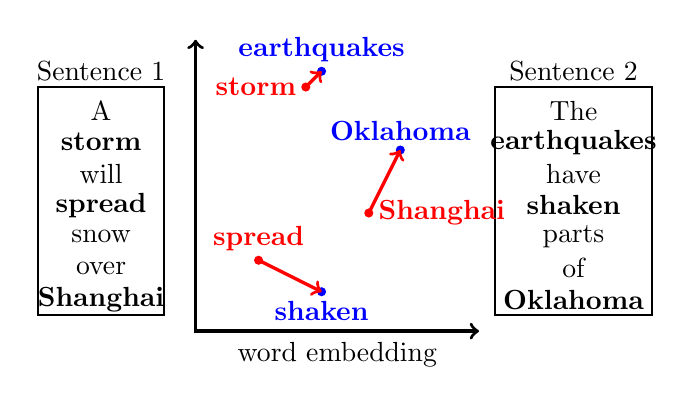
\begin{tikzpicture}
\draw [thick] (0.2, 0.5) rectangle (1.8, 3.4);
\draw [very thick, <->] (2.2, 4.0) -- (2.2, 0.3) -- (5.8, 0.3);
\draw [thick] (6.0, 0.5) rectangle (8.0, 3.4);

\node at (4.0, 0.0) {word embedding};

\node at (1.0, 3.6) {Sentence 1};
\node at (1.0, 3.1) {A};
\node at (1.0, 2.7) {\bf storm};
\node at (1.0, 2.3) {will};
\node at (1.0, 1.9) {\bf spread};
\node at (1.0, 1.5) {snow};
\node at (1.0, 1.1) {over};
\node at (1.0, 0.7) {\bf Shanghai};

\node at (7.0, 3.6) {Sentence 2};
\node at (7.0, 3.1) {The};
\node at (7.0, 2.7) {\bf earthquakes};
\node at (7.0, 2.3) {have};
\node at (7.0, 1.9) {\bf shaken};
\node at (7.0, 1.5) {parts};
\node at (7.0, 1.1) {of};
\node at (7.0, 0.7) {\bf Oklahoma};

\draw [fill, red] (3.6, 3.4) circle [radius=0.05];
\node [left, red] at (3.6, 3.4) {\bf storm};

\draw [fill, blue] (3.8, 3.6) circle [radius=0.05];
\node [above, blue] at (3.8, 3.6) {\bf earthquakes};

\draw [fill, red] (3.0, 1.2) circle [radius=0.05];
\node [above, red] at (3.0, 1.2) {\bf spread};

\draw [fill, blue] (3.8, 0.8) circle [radius=0.05];
\node [below, blue] at (3.8, 0.8) {\bf shaken};

\draw [fill, red] (4.4, 1.8) circle [radius=0.05];
\node [right, red] at (4.4, 1.8) {\bf Shanghai};

\draw [fill, blue] (4.8, 2.6) circle [radius=0.05];
\node [above, blue] at (4.8, 2.6) {\bf Oklahoma};

\draw [->, very thick, red] (3.6, 3.4) -- (3.8, 3.6);
\draw [->, very thick, red] (3.0, 1.2) -- (3.8, 0.8);
\draw [->, very thick, red] (4.4, 1.8) -- (4.8, 2.6);

\end{tikzpicture}
\caption{An illustration of the word mover's distance, an instance of micro information distance.}\label{fig:wmd}
\end{figure}
where $w_i^{S_j}$ is the word embedding of word $i$ in sentence $j$ and function $f$ is to obtain the sentence representation from word embeddings, such as sum, average or convolution. Assuming that if two sentences are similar, one word in a sentence should have the similar meaning word with another, we use the centroid of word embedding to symbolise the macro {\em INFO} of the sentence. As showed in Figure \ref{fig:wcvd}, $S_i$ represents for sentence i, and the distance between $S_1$ and $S_2$ represents for the similarity of the sentence pair. What is more, {\em storm} and {\em earthquakes} are the most important word in the sentence pair, we surely should give them more weight. As they are similar, the distance centroid tend to be close (the dashed lines). We use {\em idf} from datasets to weigh the importance.


{\em Micro Information Distance:} As for micro view, we first get the {\em INFO} of each word, and evaluate the distance between the sentence pair according to the {\em INFO} of words. The formula is described as Equation \ref{eq:micro formula}.
\begin{equation}
\tiny
\begin{aligned}
sts(S_1, S_2) = & \text{\em INFO}(w_{1}^{S_1}) + \text{\em INFO}(w_{2}^{S_1}) + \ldots + \text{\em INFO}(w_{len(S_1)}^{S_1}) \\
              - & \text{\em INFO}(w_{1}^{S_2}) - \text{\em INFO}(w_{2}^{S_2}) - \ldots - \text{\em INFO}(w_{len(S_2)}^{S_2}) \\
\end{aligned}\label{eq:micro formula}
\end{equation}
Our goal is to incorporate the semantic similarity between each word pairs into the micro information distance of sentence. Here, we adopted word mover's distance \cite{kusner2015word}, the minimum cumulative distance that all word in sentence 1 need to travel to exactly match sentence 2, showed in Figure \ref{fig:wmd}. For more details, see \newcite{kusner2015word}.


%Exprimental Setup I
{\bf Word Embedding Features:} \newcite{zhao-zhu-lan:2014:SemEval} shows that heterogenous feature outperform a single feature, and
we use three embeddings \cite{turian2010word,mikolov2013distributed,pennington2014glove} as our initial word vector input. Incidentally, the distance is substitutable, and we replace it with different measurements (i.e., {\em cosine distance, Manhanttan distance, Euclidean distance, Pearson coefficient, Spearman coefficient, Kendall tau coefficient}). Specially, because of the high time complexity of word mover's distance, we only train it on {\em word2vec} \cite{mikolov2013distributed}, although other embeddings are also plausible.

\section{Experiments}

%section overview
%In this section, we introduce our experimental methodology, including dataset, evaluation metrics and retrieval model.

\subsection{Datasets}

%To stimulate research in this area and encourage the development of creative new approaches to modeling sentence level semantics, the STS shared task has been held annually since 2012, as part of the SemEval/*SEM family of workshops. \\

We collect all the datasets from 2012 to 2015 as training data. Each dataset consists of a number of sentence pairs and each pair has a human-assigned similarity score in the range[0,5] which increases with similarity. The datasets are collected from different but related domains. We briefly describe data in Table \ref{tab:dataset}, Refer \newcite{agirre-EtAl:2015:SemEval2} for details. We emphasize dataset with symbol * for that this dataset appears both in training and test sets, which is very useful to our third submission {\bf S2} (see Section \ref{ssec:setups} for more details).
\begin{table}[h]
\tiny
\begin{center}
\begin{tabular}{crr|crr}
\hline
\hline
\multicolumn{3}{c|}{\bf{Training Set}} & \multicolumn{3}{c}{\bf{Test Set}} \\
\hline
\bf Dataset & \bf Input & \bf Gold  & \bf Dataset &  \bf Input & \bf Gold\\
\hline
\hline
MSRpar        & 1500    & 1500  & answers-answers   & 1572  & 254 \\
SMTeuroparl   & 1193    & 1193  & plagiarism        & 1271  & 230 \\
headlines*    & 3000    & 2250  & headlines*        & 1498  & 249 \\
SMTnews       & 399     &  399  & postediting       & 3287  & 244 \\
MSRvid        & 1500    & 1500  & question-question & 1555  & 209 \\
OnWN          & 2061    & 2061  & -&-&-  \\
FNWN          & 189     &  189  & -&-&-  \\
images        & 2250    &  1500 & -&-&-  \\
deft-forum    & 450     &  450  & -&-&-  \\
deft-news     & 300     &  300  & -&-&-  \\
tweet-news    & 750     &  750  & -&-&-  \\
answers-forums& 1500    &  375  & -&-&-  \\
answers-students&1500   &  750  & -&-&-  \\
belief        &2000     &  375  & -&-&-  \\
\hline
\hline
All           &19092    & 13592 & All  & 9183  & 1186 \\
\hline
\hline
\end{tabular}
\end{center}
\caption{The statistics of all datasets for STS task. Dataset with symbol * represents that this dataset appears both in training and test sets.}\label{tab:dataset}
\end{table}

\subsection{Evaluation Measurement}

In order to evaluate the performance of different algorithms, we adopt the official evaluation measure, i.e, Pearson correlation coefficient for each individual test set, and a weighted sum of all correlations is used as final evaluation metric. It weights according to the number of gold sentence pairs. The weight of a test set is equal to the rate of the gold sentences pairs in all the gold sentences.


\subsection{Learning Algorithm}
We conduct a series of experiments using all features discussed in Section \ref{ssec:traditional nlp feature engineering} and \ref{ssec:word embedding feature engineering} to obtain the optimized learning algorithm. Three supervised learning methods are explored: Support Vector Regression (SVR), Random Forest (RF) and Gradient Boosting (GB). These supervised learning algorithms are implemented using scikit-learn toolkit \cite{sklearn_api}.we use all the datasets from STS Task 2015 as development data while others from STS Task 2012 to 2014 as training data.

To configure the parameters in the regression algorithm, i.e., the trade-off parameter $c$ in SVR, the number of trees $n_{RF}$ in RF and the number of boosting stages $n_{GB}$ in GB, we make a grid search for $c$ in $[0.01, 0.1, 1, 10]$, $n_{RF}$ from $5$ to $100$ with step $5$ and $n_{GB}$ from $10$ to $300$ with step $10$.

\begin{table}[h]
\addtolength{\tabcolsep}{-1pt}
\tiny
\begin{center}
\begin{tabular}{c|ccccc|c}
\hline
\hline
\multirow{2}{*}{\bf Regression} & \multirow{2}{*}{\bf belief} & \bf answers & \multirow{2}{*}{\bf headlines} & \multirow{2}{*}{\bf images} & \bf answers & \bf Weighted \\
    & & \bf -students & & & \bf -forums & \bf Mean\\
\hline
\hline
\bf SVR(c=1) & 0.7413 &  0.7359  &  0.8168  &   0.8660  & 0.7400 & 0.7898 \\
\bf RF(n=40) & 0.7466 &  0.7100  &  0.8200  &   0.8534  & 0.7398 & 0.7816 \\
\bf GB(n=140)& \bf 0.7655 &   0.7484  &  \bf 0.8439  &   \bf 0.8791  & \bf 0.7469 & \bf 0.8080 \\
\hline
\hline
\bf DLSCU-S1 & 0.7491 &  \bf 0.7725  &  0.8250  &   0.8644  & 0.7390 & 0.8015 \\
\hline
\hline
\end{tabular}
\end{center}
\caption{Pearson coefficient of development data using different algorithms with different hyperparameter, as well as top rank results on STS 2015 test data.} \label{tab:algorithmSelection}
\end{table}
Table \ref{tab:algorithmSelection} shows the best result of each algorithm , as well as the top runs on STS 2015 test data. GB(n=140) outperformed other algorithms on all datasets. We choose GB(n=140) as our final regression algorithm on our next series experiments. Also, without any specific training dataset selections or choosing suitable features, we achieve the considerable results compare to the top runs on STS 2015 Task. \newcite{sultan-bethard-sumner:2015:SemEval} has shown that specific training datasets with similar domains and enough data will yield better results than an all-inclusive training datasets. And next we endeavor to select specific training sets and suitable features.

\subsection{System Setups}
\label{ssec:setups}
We build three different systems according to the usage of training datasets as follows.

{\bf U-SEVEN:}
This is an unsupervised system based on the word aligner described in \cite{sultan-bethard-sumner:2015:SemEval} without any training data. We evaluate semantic similarity by adopting straight-forward measurements (i.e., longest common sequence, alignment feature, corpus-based feature, all four features from word embedding features), which are averaged to get the final score. We adopt {\em  cosine distance, Pearson coefficient, Spearman coefficient} as the distance measurements, which perform better results on our preliminary experiments.
%As to distance function in word embedding features, {\em  cosine distance, Pearson coefficient, Spearman coefficient} are selected, which is based on our experiments on all datasets, where these subsets yield better results than an all-inclusive training set (seemingly due to the range of these measurements are similar).
%In this section, we assess the effectiveness of our proposed models for Similarity Measure. In particular, we aim to answer the following research questions:

{\bf S1-All:}
We use all the training datasets and build a single global regression model regardless of domain information of different test datasets. In order to make better use of these features and improve the performance, we construct feature selection procedure on development set (i.e., test set of STS 2015 Task) and vote for the preserved feature sets. As for feature selection strategy, we adopt {\em hill climbing}: keep adding one type feature at a time until no further improvement can be achieved.

{\bf S2:}
\newcite{sultan-bethard-sumner:2015:SemEval} has shown that taking all the training datasets into consideration may hurt the performance since training and test sets are from different domains. Hence, for each test set, we select the datasets which are most similar, taking source, average length of sentences and word mover's distance (discussed in Section \ref{ssec:word embedding feature engineering}) into consideration. For the data set with symbol * (i.e., {\em headlines}), we use all {\em headlines} pairs.  For {\em answers-answers} and {\em question-question}, we use {\em belief, deft-forums, answers-students, answers-forums} pairs. For postediting, we use {\em SMTeuropar} and {\em MSRpar} pairs. For plagiarism, we use {\em onWN} and {\em FNWN} pairs.


\section{Results on Training Data}
According to the above preliminary experimental results, we employ GB(n=140) algorithm as our final regression algorithm. In order to explore the influences of word embedding features and make better use of all the above features, we construct feature selection experiment on development set (i.e., test set of STS 2015 Task) and vote for the preserved feature sets.

\begin{table}[h]
\addtolength{\tabcolsep}{-3pt}
\tiny
\begin{center}
\begin{tabular}{cl|c|c|c|c|c}
\hline
\hline
\multicolumn{2}{c|}{\multirow{2}{*}{\bf Feature}} & \bf \multirow{2}{*}{belief} & \bf answers & \bf \multirow{2}{*}{headlines} & \bf \multirow{2}{*}{image} & \bf answers \\
   &    &   & \bf -students &   &   & \bf-forums \\
\hline
\hline
\multirow{5}{*}{\bf String-based}   & len   &     -   &  -      & $\surd$ & $\surd$ &  -        \\
                                    & pos   &     -   &  -      & $\surd$ & -       & $\surd$   \\
                                    & lcs   &     -   &  -      & $\surd$ & $\surd$ & $\surd$   \\
                                    & $n$-grams &     -   & $\surd$ & $\surd$ & $\surd$ & $\surd$   \\
                                    & ner   &     -   & $\surd$ & $\surd$ &  -      &  -         \\
\hline
\multirow{2}{*}{ \tabincell{c}{\bf Machine\\ \bf Translation}}
                                    & average& $\surd$&  -      & $\surd$ & $\surd$ &  -        \\
                                    & concat&     -   &  -      &  -      &    -    &  -        \\
\hline
\multirow{2}{*}{\bf Corpus-based}   &wordnet&$\surd$  & $\surd$ & $\surd$ &  -      & $\surd$   \\
                                    & lsa   &     -   & $\surd$ & $\surd$ & $\surd$ & $\surd$   \\
\hline
\multirow{2}{*}{\bf Alignment}      & global&     -   & $\surd$ & $\surd$ & $\surd$ & $\surd$   \\
                                    & pos-specific&$\surd$& $\surd$ & $\surd$ & $\surd$ & $\surd$   \\
\hline
\hline
\multirow{3}{*}{ \tabincell{c}{\bf Word Embedding \\ \bf (Macro)} }\
                                    & word2vec&$\surd$& $\surd$ & $\surd$ & $\surd$ & $\surd$   \\
                                    & glove   &   -   &    -    &  -      & -       &  -        \\
                                    & turian's&$\surd$& $\surd$ & $\surd$ & $\surd$ &  -        \\
\hline
\tabincell{c}{\bf Word Embedding \\ \bf (Micro)}
                                    & wmd     &$\surd$& $\surd$ & $\surd$ & $\surd$ & $\surd$   \\
\hline
\hline
\multicolumn{2}{c|}{\bf Our Results} & \bf 0.7835 & 0.7713 & \bf 0.8455 & \bf 0.8808 & \bf 0.7636 \\
\hline
\multicolumn{2}{c|}{\bf Best Scores}  & 0.7717 & \bf 0.7879 & 0.8417 & 0.8713 & 0.7390 \\
\hline
\hline
\end{tabular}
\end{center}
\caption{Results of feature selection experiments on STS 2015 test data. The last row shows the the best scores of all submitted system on STS 2015 task.}
\label{tab:train}
\end{table}
% word Embedding Feature can improve performance, micro and macro are not conflict, combine of can improve the performance
% specific aligned feature can �ֲ� global �IJ���
% contact and glove not perform well on each set, remove it

Table \ref{tab:train} shows the results of feature selection experiments on STS 2015 test data. From the table, we find that 1) Word embedding features, the positive complementary of macro perspective and micro perspective, indeed improve results. 2) Specific alignment features can compensate for the weaknesses of global alignment features. 3) Since concatenate MT metrics and glove features does not perform well on all five data sets, we remove them from our feature sets and train our S1-All model with the preserved features.
%{\color{red} reason of MT and glove fail.}

\section{Results on Test Data}

%compare the three system, all performance , em S1-All and U-SEVEN, analysis S2
%analysis the result on answer-answer, example, reason(the struct is sim while mean is different, focus on the different and focus on the key center)
Table \ref{tab:test} summarizes the results of our submitted runs on test datasets officially released by the organizers, as well as the top runs. In terms of weighted mean of Pearson measurement, system S1-All performs the best while our corpus-specific system {\bf S2} performs the worst. We think the measurement to choose training data from the candidate datesets in main task are ill-suited. It is noteworthy that on plagiarism and postediting, our unsupervised model U-SEVEN achieves much better results than the supervised model (i.e., S1-All, S2), which indicates the efficiency of the ensemble of similar measurements.

\begin{table}[h]
\scriptsize
\begin{center}
\begin{tabular}{c|ccc|c}
\hline
\hline
\multirow{2}{*}{\bf Dataset} & \multicolumn{3}{c|}{\bf Runs}  & \bf Best \\
                              \cline{2-4}
                              & \bf U-SEVEN & \bf S1-All & \bf S2 & \bf Score \\
\hline
\hline
\bf answers-answers &     0.4774  &     0.5697 & \bf 0.5715 & 0.6923\\
\bf plagiarism      & \bf 0.8301  &     0.8250 &     0.7733 & 0.8413\\
\bf headlines       &     0.7668  & \bf 0.8121 &     0.7903 & 0.8274\\
\bf postediting     & \bf 0.8423  &     0.8234 &     0.7496 & 0.8669\\
\bf question-question&    0.7191  & \bf 0.7311 &     0.6763 & 0.7470\\
\hline
\hline
\bf weighted mean   &     0.7242  & \bf 0.7507 &     0.7116 & 0.7780\\
\hline
\hline
\end{tabular}
\end{center}
\caption{The results of our three runs on STS 2016 test datasets.The rightmost column shows the best score by any system. The last row shows the value of the officially evaluation metric.}\label{tab:test}
\end{table}
On {\em answer-answer} set, the gap between top systems and our systems is about 12\%. According to our investigations on this set, we find that certain sentence pairs are similar in syntactical structure but express different meanings. For example,
\begin{displaymath}
\left\{ \begin{array}{ll}
\text{\em You should do it.}\\
\text{\em You can do it, too.} \\
\end{array} \right.
\left\{ \begin{array}{ll}
\text{\em It's pretty much up to you.}\\
\text{\em It's much better to ask.} \\
\end{array} \right.
\end{displaymath}
Our assumption (i.e., two sentences with similar syntax structure convey similar meaning) does not apply to the above condition.

\section{Conclusion}


%how do? achieve what? result analysis? conclusion? future work?
%focus on the different and focus on the key center)
%word embedding features is highly interpretable
We use the traditional NLP features including string-based features, corpus-based features and alignment features for textual similarity estimation, as well as efficient word embedding features. It is also worth pointing out that our word embedding features are highly interpretable and hyper-parameter free, as well as they are straight-forward to measure semantic textual similarity. The difference between top system and our best system is about 2.8\%, which means our systems are promising. Noticing the gap between top system and our systems on {\em answer-answer} set, we will explore to find the central words of sentences in future work.

\section*{Acknowledgments}

This research is supported by grants from Science and Technology Commission of Shanghai Municipality (14DZ2260800 and 15ZR1410700), Shanghai Collaborative Innovation Center of Trustworthy Software for Internet of Things (ZF1213).


\bibliography{en-acl-template}
\bibliographystyle{naaclhlt2016}

\end{document}
